\newpage

\section{Best Practices}



\subsection{Coding}
\begin{itemize}
	\item Draw your schematics/state machines on paper before coding!
	\begin{itemize}
		\item Do not try to save paper!
		\item Clearly mark combinational logic in one color and non-combinational in another. 
\item leave out clocks and resets from your drawing... too messy	
	\end{itemize}
	\item Make one separate file for each module. Recommended granularity: A stage is a module, e.g. "execute.v, decode.v, ..." This split is actually finer-grained than absolutely necessary, but gives a nice, clean design.\\
	\item Instantiate all synthesizable modules within "cpu.v". Then instantiate "cpu.v" in ''testbench.sv". This gives a nice, clean structure.
	\begin{center}
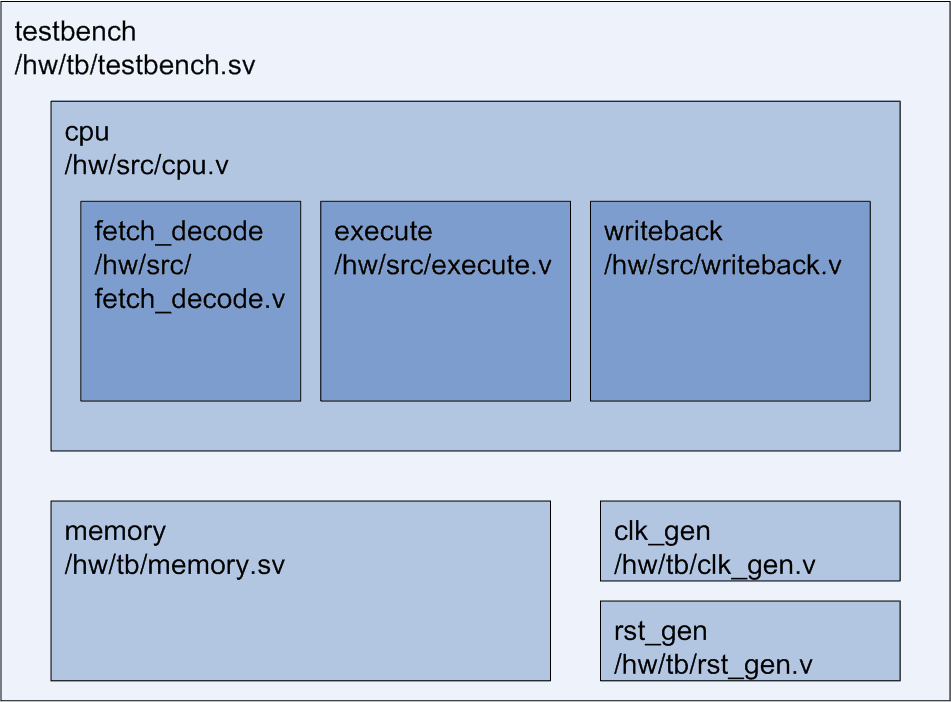
\includegraphics[width=6cm]{figs/block}
\end{center}
	\item Register all outputs of each stage, i.e. the output is driven by a register directly!
\begin{center}
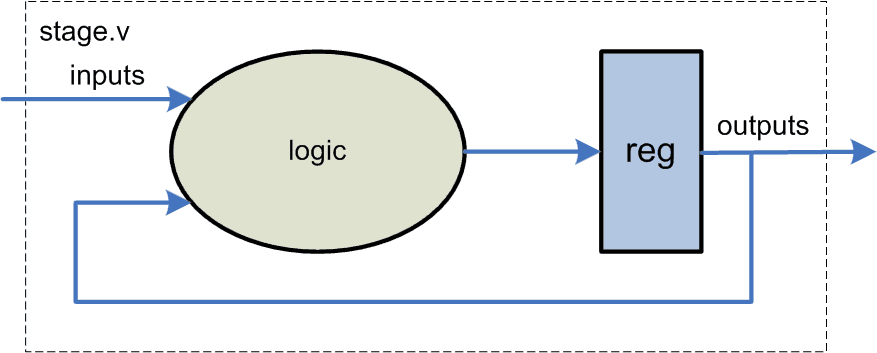
\includegraphics[width=6cm]{figs/stage}
\end{center}
This ''latched mealy'' machine is a very fast and safe technique to model pipelined data paths. (Mealy and Moore are taught in classes because they are difficult enough to confuse students. They are rarely used though, because of some poor properties: When connected together Mealy machines produce long combinational paths. Moore does not yield such long combinational paths but the basic drawback remains.)\\
%	Note 1: Inputs to a stage may be the outputs of any stage.\\
%	Note 2: Think twice whether you need a Mealy or Moore machine in your design.\\
%In short: One stage has inputs on the left, followed by combinational logic, followed by registers, followed by outputs.

	\item Decide upon a naming convention for signals, registers, modules, constants,...! Consistency helps when your code base grows larger and larger.
	\item Do not reinvent the wheel: Use the built-in operators ''+'' and ''-'' for addition and subtraction. The synthesis tool will infer the right architecture for you.
	\item No tri-state buses and no ''inout'' ports
	\item Port connections only by name, not by position
	\item Tasks/functions only if absolutely necessary
	\item Save your files often (at least once before lunch break and before leaving in the evening)! You can use a revision control system if you like.
	\item Comments, comments, comments
\end{itemize}


\subsection{Tools}
\begin{itemize}
	\item Do not run any tool in the same working directory in two shells at the same time. Instead have seperate working directories for each instance of the respective tool.
	\item Use the graphical user interface (GUI) to get familiar with the functionality. Later, you can observe the commands issued by the GUI to create your own scripts. The latter is preferred because it guarantees reproducibility. Also many useful commands/options are not available in the GUI.
\end{itemize}

\subsection{Group Work}
	\begin{itemize}
	\item Work together, discuss regularly and often.
	\item At least once a day (in the morning), discuss what each of you will do today.
	\item Work in pairs of 2 for a while, then come together to integrate your work. Explain what you did to the others. Make only small iterations!
	\item Make only small iterations! REALLY!
	\item Inform each other of your schedules/absences well in advance.
	\end{itemize}